
\documentclass[a4paper, 10pt]{IEEEconf}  

\usepackage{geometry}
\geometry{a4paper, margin=1in}
  
  
\usepackage{subcaption}  
\usepackage[export]{adjustbox}    
\usepackage{verbatim}
\usepackage{graphicx}
\usepackage{pdfpages}
\usepackage{cite}
\usepackage{listings}
\usepackage{float}
\usepackage{url}
\usepackage{hyperref}
\usepackage{fancyhdr}
\usepackage{multicol}

\lstset{
	tabsize=2,
	breaklines=true
}

\setlength{\parskip}{1em}
\onecolumn

\title{\LARGE \bf Assignment 2: Orienteering Optimisation\\Simulation Modelling and Optimisation 282 758}
\author{Marc Alexander Sferrazza \\ 12164165
\thanks{This work was not supported by any organization}
\thanks{Faculty of Mechatronics Engineering, Massey University, Albany, Auckland, New Zealand
        {\tt\small Progress of project: https://github.com/alex1v1a/Simulation-Modelling-and-Optimisation/} } }

\begin{document}

\maketitle
\begin{figure}[h]
\begin{subfigure}{\textwidth}
\includegraphics[width=\textwidth, center]{images/points} 
%\caption{ROS}
%\label{fig:ROS}
%\end{subfigure}
%\begin{subfigure}{0.5\textwidth}
%
\includegraphics[width=0.3\textwidth, right]{images/gazebo}
%\caption{Gazebo} 
\label{fig:Gazebo}
\end{subfigure}
%\caption{Caption for this figure with two images}
%\label{fig:image2}
\end{figure}
\begin{figure}[H]
  \begin{center}
  
\includegraphics[width=\textwidth]{images/masseyUniversity}
  \label{fig:kinetic}
  \end{center}
\end{figure}
\thispagestyle{empty}
\pagestyle{plain}


%%%%%%%%%%%%%%%%%%%%%%%%%%%%%%%%%%%%%%%%%%%%%%%%%%%%%%%%%%%%%%%%%%%%%%%%%%%%%%%%

%\begin{abstract}

%In this assignment you will setup ROS on your computer and install Gazebo simulator. ROS has a number of robot models ready for using in Gazebo, of which you can choose one and link it to main ROS packages for tele-operation from your keyboard. Add a laser scanner (e.g. Hokuyo URG or Sick Scanner) to the robot making sure the scanner publishes laser data over ROS. One choice of the robot model could be Poineer-3DX which is also available in hardware form. Your simulated code will run on the real robot without modification.

%\end{abstract}


\clearpage
\thispagestyle{empty}
\tableofcontents
\begingroup
\let\clearpage\relax
\listoffigures
%\listoftables
\endgroup
%\thispagestyle{empty}
\clearpage
\twocolumn

%%%%%%%%%%%%%%%%%%%%%%%%%%%%%%%%%%%%%%%%%%%%%%%%%%%%%%%%%%%%%%%%%%%%%%%%%%%%%%%%
%%%%%%%%%%%%%%%%%%%%%%%%%%%%%%%%%%%%%%%%%%%%%%%%%%%%%%%%%%%%%%%%%%%%%%%%%%%%%%%%
\clearpage
\setcounter{page}{1}
%\thispagestyle{empty}
\onecolumn

\section{INTRODUCTION}

An orienteering course has a number of controls that can be reached. The task is to optimise the result for various running speeds on which a runner can attempt to complete the course, based on a certain points scheme. Using a branch of optimisation called evolutionary optimisation, the GAOT (genetic algorithm optimisation toolbox - 1995) is to be implemented, to take advantage of it's class, or group of optimisation techniques. The Biological evolution techniques are modelled in Matlab and results extracted to this report.

%%%%%%%%%%%%%%%%%%%%%%%%%%%%%%%%%%%%%%%%%%%%%%%%%%%%%%%%%%%%%%%%%%%%%%%%%%%%%%%%

\subsection{Overview}
The orienteering course is shown below and the target points values are worth either 2, 3 or 4 points. There are 27 controls total, 9 of each worth 2, 3, and 4 points respectively. Runners have 60 minutes to maximise their score with a penalty of 2 points per 30 seconds late back. 

The constraints and limitations indicate that a runner must remain on the yellow marked paths at all times during the simulation, to otherwise therefore not cross any private grounds, and/or walk through buildings etc. 

\begin{figure}[H]
  \includegraphics[width=\linewidth, center]{images/points}
  \caption{Terrace End School Points Course}
  \label{fig:Terrace End School Points Course}
\end{figure}

%%%%%%%%%%%%%%%%%%%%%%%%%%%%%%%%%%%%%%%%%%%%%%%%%%%%%%%%%%%%%%%%%%%%%%%%%%%%%%%%
%%%%%%%%%%%%%%%%%%%%%%%%%%%%%%%%%%%%%%%%%%%%%%%%%%%%%%%%%%%%%%%%%%%%%%%%%%%%%%%%
\clearpage
\section{METHOD}

The Matlab model to be presented is based on Setup Code*, Opt Function, Objective function* 

After locating the control points on the map and their respective distances to one another on a legal term based from the constraints; the points are then translated to an array matrix which can be used to easily lay all possible distances to each point in all combinations, of which 729 terms are found.

From the combinations of distances the Genetic Algorithm function can be used to calculate the optimal route for runner based on the given speed, with the shortest distance.

%%%%%%%%%%%%%%%%%%%%%%%%%%%%%%%%%%%%%%%%%%%%%%%%%%%%%%%%%%%%%%%%%%%%%%%%%%%%%%%%

%\subsection{Block Diagram of running model}

%%%%%%%%%%%%%%%%%%%%%%%%%%%%%%%%%%%%%%%%%%%%%%%%%%%%%%%%%%%%%%%%%%%%%%%%%%%%%%%%

\subsection{Genetic Algorithms}
Using a Genetic Algorithm the method of natural selection (Darwinism - Survival of the fittest, or in this case best performance) can been deemed appropriate based on the biological evolution techniques described in the search algorithm. Therefore applying this technique to the 27 combinational control options the runner can achieve in 60 min, the maximum score can be calculated by simulation of exclusions to the weakest links.

Eventually the model will find the optimal solution based on the runners speed after shedding all other less efficient options, like that of the process of natural evolution systems. It does this based on a randomised search; however while the method is randomised the past results and background informations are used to find a region of interest with best performance, to narrow the scope of the search and find a optimal result in a faster given time.

%%%%%%%%%%%%%%%%%%%%%%%%%%%%%%%%%%%%%%%%%%%%%%%%%%%%%%%%%%%%%%%%%%%%%%%%%%%%%%%%

\subsection{Distance and Coordinates Allocation}

Using Google maps the distances are recorded from each control point, traveling centred along each path and scaled accordingly. In order to set up the Genetic Algorithm the distances are then translated to a matrix with every possible distance from each control device mapped (27x27 array of 729 terms) - The matrix then is converted to the shortest distances between controls.

%%%%%%%%%%%%%%%%%%%%%%%%%%%%%%%%%%%%%%%%%%%%%%%%%%%%%%%%%%%%%%%%%%%%%%%%%%%%%%%%

\subsection{Tracker Function}

Please note the orderBasedExample has been used with tspEval (modified to tracker) from the GAOT toolbox for this section.

To find the shortest route for the runners the Genetic Algorithm function needs to be called, but scoring for each point must be taken into consideration and therefore implemented with the Genetic Algorithm function. (Please see fig. orderBasedExample)

The adaptive aspect of the function loops and gets results for every iteration in the target, scores are added and the acquired distance based on a rotated location is incremented on the common term. The input passed is the runners speed; other inputs and outputs are also available like the obvious total points or final score. The scores are added - there are 9 of each, 2, 3 and 4 - when the runner reaches each control formed on a coordinate list. The cycle continues until the position doesn't change then exits, where the position is overwritten and run again until the loop is complete.

The penalties are then deducted from the total score after the 60 min time limit is reached, a 2 point reduction is taken per 30 seconds the runner returns late. (Please refer to fig. tracker with commentary for further details)

A full code snippet has been provided in the appendix for full step by step details please review comments, also a full version of the .m files have been attached for reference.

%%%%%%%%%%%%%%%%%%%%%%%%%%%%%%%%%%%%%%%%%%%%%%%%%%%%%%%%%%%%%%%%%%%%%%%%%%%%%%%%
\clearpage
\subsection{Optimisation Process}
Using the GAOT toolbox there is a function to process optimisation based on a genetic algorithm technique. The orderBasedExample.m and tspEval.m files have been modified to fit the model accordingly. 

By loading the array of data points (distances between coordinates) that have been found on the orienteering map, it is then necessary to use the y axis's size in order to calculate the bounds. 

To begin the sequence a route must be chosen, this is done in the startpop variable where the initalizeoga function is called, which passes back 200 randomly selected routes.

With this method it is possible to set the limit of how many trials will be simulated, this can be done using the termOps variable and will be the suggestion of the amount of generations to simulate which are 20 in this case.

The tspEval function has been modified to score the populations results and find the best values, doing so based on previous trials values to be selected from the genetic algorithm, in this instance the function has been named tracker to be called be the orberBasedExample.m

%%%%%%%%%%%%%%%%%%%%%%%%%%%%%%%%%%%%%%%%%%%%%%%%%%%%%%%%%%%%%%%%%%%%%%%%%%%%%%%%
%%%%%%%%%%%%%%%%%%%%%%%%%%%%%%%%%%%%%%%%%%%%%%%%%%%%%%%%%%%%%%%%%%%%%%%%%%%%%%%%
\section{RESULTS}

The genetic algorithm finds the best possible path (this result may vary due to the nature of the algorithm), and the tracker function calculates the score for each path. The outputs given from the ga function are ga, x, endpop, bestpop, and trace - x is a 29 bit array of the 28 steps taken along the optimal path found for this population set and trial at hand. The last value in the set is the relevant score for the path.

The following arguments received, endPop (generations 200x29) for finding the combination of the best score for this route, bestPop (possible results), and trace which gives information such as mean and standard deviation of the generations along with the best score. 

%\begin{figure}[H]
%  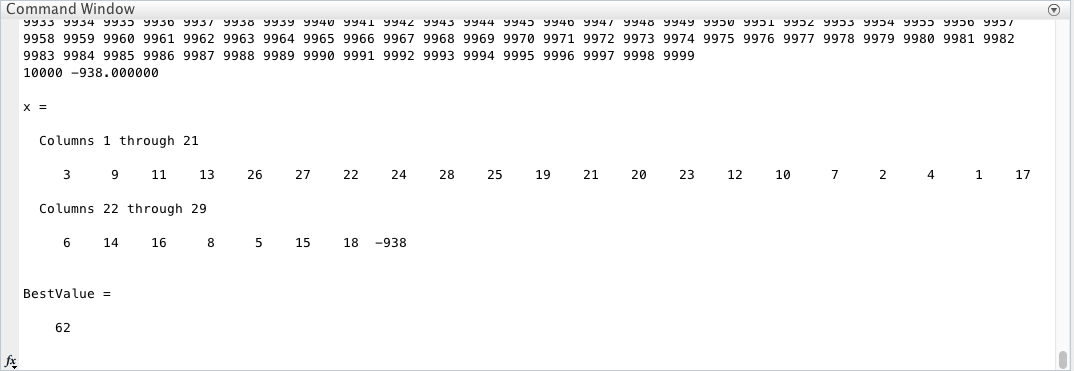
\includegraphics[width=\linewidth, center]{images/score}
%  \caption{Results produced from Matlab, scores}
%  \label{fig:Results produced from Matlab, scores}
%\end{figure}

A mapped figure of the paths are shown below. The trail of dotted blue indicates each generations path, while the red shows the optimal path.

%\begin{figure}[H]
%  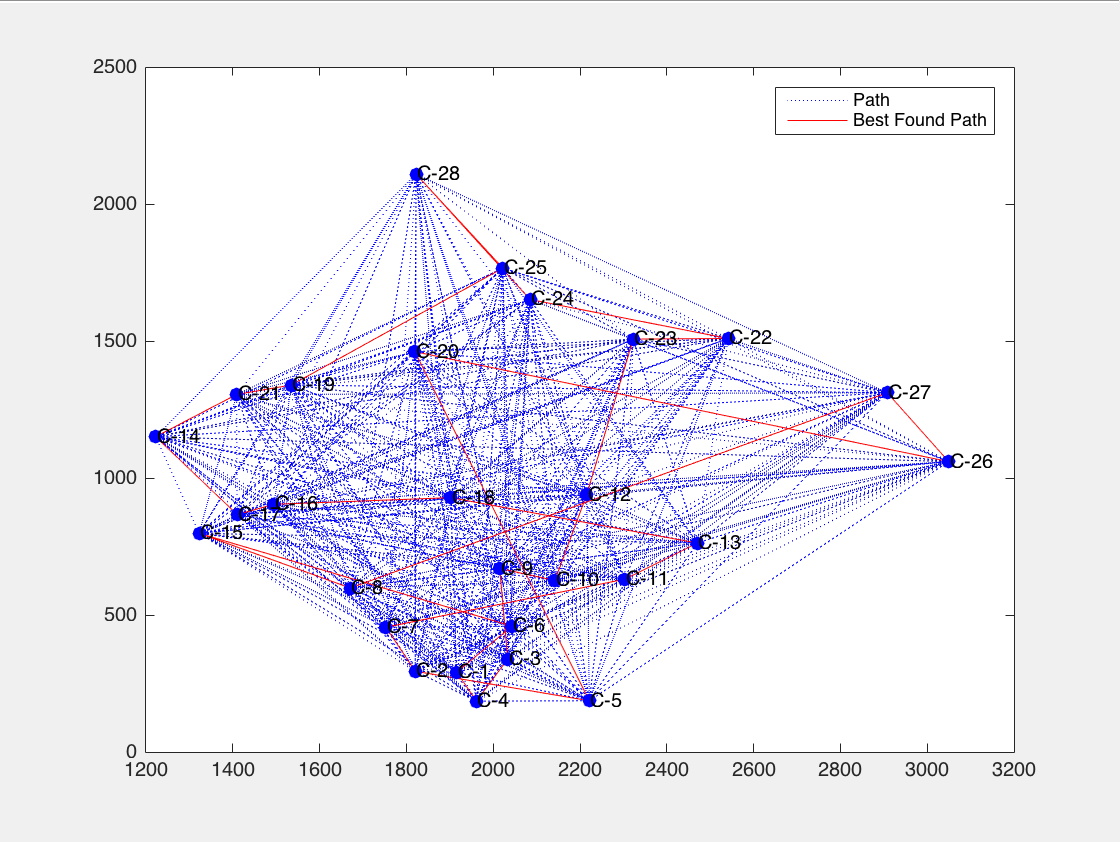
\includegraphics[width=\linewidth, center]{images/path}
%  \caption{A map of paths taken and best path found}
%  \label{fig:A map of paths taken and best path found}
%\end{figure}

%%%%%%%%%%%%%%%%%%%%%%%%%%%%%%%%%%%%%%%%%%%%%%%%%%%%%%%%%%%%%%%%%%%%%%%%%%%%%%%%
%%%%%%%%%%%%%%%%%%%%%%%%%%%%%%%%%%%%%%%%%%%%%%%%%%%%%%%%%%%%%%%%%%%%%%%%%%%%%%%%

%\section{OUTCOMES}


%%%%%%%%%%%%%%%%%%%%%%%%%%%%%%%%%%%%%%%%%%%%%%%%%%%%%%%%%%%%%%%%%%%%%%%%%%%%%%%%
%%%%%%%%%%%%%%%%%%%%%%%%%%%%%%%%%%%%%%%%%%%%%%%%%%%%%%%%%%%%%%%%%%%%%%%%%%%%%%%%
\clearpage
\section{CONCLUSIONS}

For any progress related to the assignment please see the public Github repo for alex1v1a or use the link in the cover page to be automatically redirected to this project. The repo provides all relative project information.

Using the genetic algorithm it is feasible to find optimal results for a given population input, which can be applied to a vast range of scenarios from things small like DNA, or larger groups as talked about in this example. The implementation of this algorithm and inputs passed to the functions are used to find the optimal path for an orienteering runner are generated to provide the highest results provided the highest score is achieved in the fastest time. 

The results give the optimal values for this particular solution to the effect of which are suitable for only this example. The process can be run for different instances by adjusting the population and trial values but the distances for each control point remain the same therefore the method used may not be the most efficient for this example as the distances are fixed along with the speed, points and other remaining factors of the example.               

%%%%%%%%%%%%%%%%%%%%%%%%%%%%%%%%%%%%%%%%%%%%%%%%%%%%%%%%%%%%%%%%%%%%%%%%%%%%%%%%
%%%%%%%%%%%%%%%%%%%%%%%%%%%%%%%%%%%%%%%%%%%%%%%%%%%%%%%%%%%%%%%%%%%%%%%%%%%%%%%%

%\nocite{*}
%\bibliographystyle{ieeetr}
%\bibliography{references}

%%%%%%%%%%%%%%%%%%%%%%%%%%%%%%%%%%%%%%%%%%%%%%%%%%%%%%%%%%%%%%%%%%%%%%%%%%%%%%%%
%%%%%%%%%%%%%%%%%%%%%%%%%%%%%%%%%%%%%%%%%%%%%%%%%%%%%%%%%%%%%%%%%%%%%%%%%%%%%%%%

%\clearpage
%\onecolumn
%
\section*{APPENDIX}

\begin{figure}[H]
  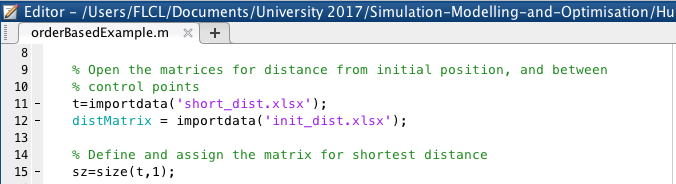
\includegraphics[width=\linewidth, center]{images/import}
  \caption{Import the dist matrices to orderBasedExample}
  \label{fig:Import the dist matrices to orderBasedExample}
\end{figure}

\begin{figure}[H]
  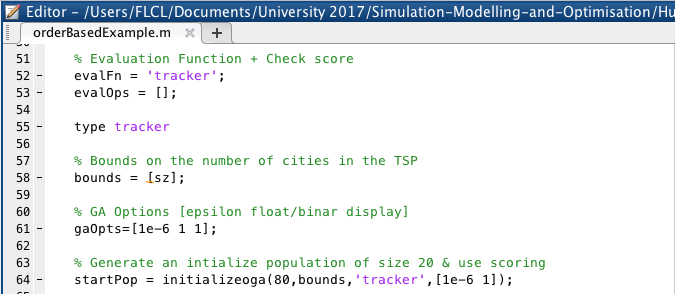
\includegraphics[width=\linewidth, center]{images/scoring}
  \caption{Preform Genetic Algorithm and call function "tracker" for scoring}
  \label{fig:Preform Genetic Algorithm and call function "tracker" for scoring}
\end{figure}

\begin{figure}[H]
  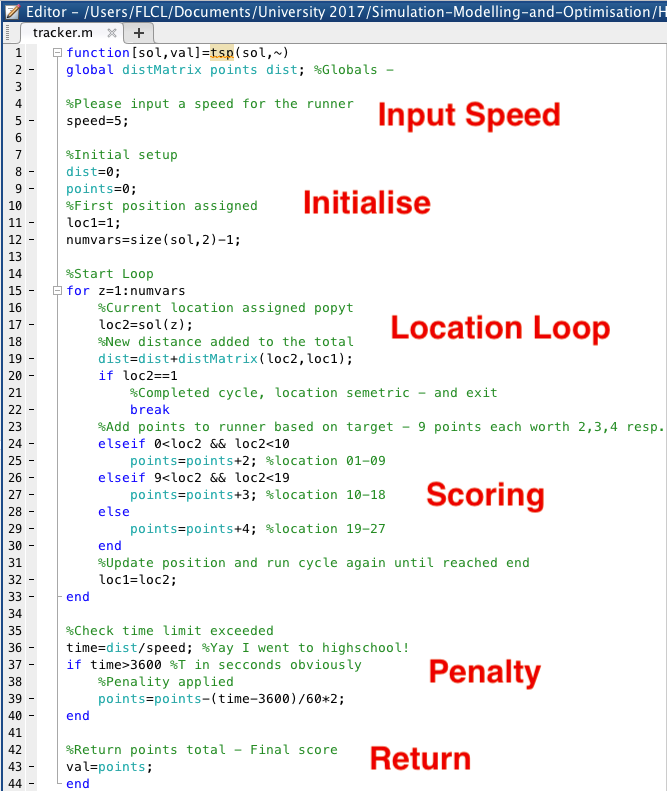
\includegraphics[width=\linewidth, center]{images/tracker}
  \caption{Tracker function, used to check position and calculate points \\ Note Penalty changed to 30 seconds (stream error before screenshot taken and edited)}
  \label{fig:Tracker function, used to check position and calculate points}
\end{figure}


\end{document}
